\begin{table}
	\begin{tabular}{c|c|c|c}
	\hline
Form & String & Feature & AR \\ \hline 
		\makecell{ \textit{mù.tûm} \\ `person'}	 & L.HL & \makecell{+L\\-C} .\makecell{-L\\-C}\makecell{+L\\-C}&
		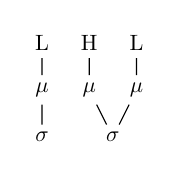
\begin{tikzpicture}
			[scale=0.6, every node/.style={scale=0.8}]
			\node (t0) at (1,1) {L};
			\node (t1) at (2,1) {H};
			\node (t2) at (3,1) {L};
			\node(c1) at (1,0) {$\mu$};
			\node(c2) at (2,0) {$\mu$};
			\node(c3) at (3,0) {$\mu$};
			\node (s1) at (1,-1) {$\sigma$};
			\node (s2) at (2.5,-1) {$\sigma$};
			\draw (t0) -- (c1) -- (s1);
			\draw (t1) -- (c2) -- (s2);
			\draw (t2) -- (c3) -- (s2);
		\end{tikzpicture} \\ \hline
 (nonce)	 & R.H &  \makecell{+L \\ +C} .\makecell{-L \\ -C}&
		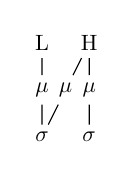
\begin{tikzpicture}
			[scale=0.6, every node/.style={scale=0.8}]
			\node (t0) at (1.5,1) {L};
			\node (t1) at (2.5,1) {H};
			\node(c1) at (1.5,0) {$\mu$};
			\node(c2) at (2,0) {$\mu$};
			\node(c3) at (2.5,0) {$\mu$};
			
			\node (s1) at (1.5,-1) {$\sigma$};
			\node (s2) at (2.5,-1) {$\sigma$};
			\draw (t0) -- (c1) -- (s1);
			\draw (t1) -- (c2) -- (s1);
			\draw (t1) -- (c3) -- (s2);
		\end{tikzpicture} \\ \hline
	\end{tabular}
	\caption{Positive and Negative forms in three representations}
	\label{tab.threereps}
\end{table}

